
\documentclass[journal]{IEEEtran}
\usepackage{blindtext}
\usepackage{graphicx}

\ifCLASSINFOpdf
\else
\fi

\hyphenation{op-tical net-works semi-conduc-tor}


\begin{document}


\title{spAAce: an application for controlling sound source movements in a Wavefield Syntehsis system}


\author{Diego Di Carlo ddicar16@student.aau.dk,
        Jorge Madrid Portillo jmadri15@student.aau.dk,
        Matteo Girardi mgirar15@student.aau.dk%
}


\markboth{Journal of \LaTeX\ Class Files,~Vol.~6, No.~1, January~2007}%
{Shell \MakeLowercase{\textit{et al.}}: Bare Demo of IEEEtran.cls for Journals}


\maketitle


% This is the also the 'conclusion'
\begin{abstract}
We present a graphical application called \emph{spAAce} which let users control real-time movements of sound sources by drawing trajectories. The first prototype of this application has been developed for a Wavefield Synthesis Systems and it is bound with WFSCollider, an open-source software based on Supercollider which let users handle such synthesis technique. In order to communicate with such software the Open Sound Control protocol has been employed. The \emph{spAAce} application has been implemented using Processing, a programming language for sketches and prototypes within the context of visual arts. This application aims to create a new way of interaction for live performance of spatial composition and live electronics.
\end{abstract}

\begin{IEEEkeywords}
Wavefield Synthesis, WFSCollider, spAAce, spatial music composition, Processing.
\end{IEEEkeywords}

\IEEEpeerreviewmaketitle

\section{Introduction}
The spatial characteristic of a composition has been an important topic for the avant-garde musicians in the past decades \cite{MusikImRaum} and it still is a relevant quality of a musical piece \cite{baalman2003application}. From an artistic point of view, conveying spatial musical ideas and thoughts could underestimate the technical issues that must be faced during the development and implementation process of a software for musical purposes. Hence, contemporary composers and sound engineers have to find a trade-off during such process of composing new musical material. Moreover, learning new technologies or softwares for spatial music could be time consuming for composers that do not have a deep knowledge in the computer music field. Therefore, the \emph{spAAce} application attempts to provide the following advantages:
\begin{enumerate}
\item a quick way to sketch and test movements of sound sources.
\item improvisation with spatial sound sources during live performances.
\end{enumerate}
The latter point could lead to new approaches of performing live concerts in a live electronics scenario. Indeed, WFSCollider is employed just as engine render while the composers can focus on creating trajectories for sound sources and expanding musical expression.

\subsection{State of the art}
Many different softwares for spatial sound movements have been developed in the recent years \cite{jot95} \cite{wfsc} \cite{geier12} and several spatial techniques have been implemented such as VBAP, DBAP, Ambisonics and Wavefield synthesis (WFS). 
% WFS and WFSCollider: what is it, why we use it? IT IS FREE!
Most of the spatial rendering engines come with an graphical user interface, such as SoundScape Render \cite{geier12}, Spat \cite{jot95}, WFSCollider \cite{wfsc} itself and many others. However they are more focused of the rendering side, lacking of a proper interface that a composer or an artist can intuitively use to convey their creativity. With the spreading of user-friendly GUI development environments for mobile and web app, lots of client application have been developed for these rendering engines, which allow real-time finger-based interaction. Some of them are more are mixing-oriented, providing a real-time positioning of the sound sources in the space, while others, such as Trajectoires \cite{favory15} and Spatium \cite{penha13}, allow the users to move the sound sources and create complex paths both in time and in space.
However, these new applications are still in the embryonic stage and there is a lot of work still to be done in order to design the most suitable interface that can capture the actual intentions of the performers. The key concept of \emph{spAAce} is the combination of several modes of interaction that should encourage and enable artistic sound spatialization.
% Similar project:
% Trajectory (web client for Spat~) <::: IRCAM Paris
% spaceJam (GUI for MAX) <::: Adriana New York 
% ViMiC (Max develop with Jamoma and plugIn for Audio Unit) <::: McGill University
% SpatDIF (C++, Max external, Openframework) <::: ZHdK ICMST
% Spatium (interface and render for Max and Audio Unit, some gui in processing) <::: Rui Penha
% Android Client for SoundScape Render <::: TUB Berlin


% MATERIAL AND METHODS SECTIONS:
\section{Design process}
Gathering knowledge about the current state of the art has been a necessary step in order to have a clear view on this topic. Knowing what kind of technologies are usually employed, the development path has led us to employ Processing \cite{processing} as development platform, since it has many libraries and a strong community of developers. 
% \subsection{Interview}
The next step has been asking composers and sound engineers for interviews to propose the main concept of the \emph{spAAce} application in order to test if there was actually a reason to start developing such software and to have general feedback, hints and suggestions. These composers and sound engineers are highly involved in contemporary music production and live electronics performances. These interviews gave a solid starting point to implement the main core of the application. An iterative procedure of implementation-testing-fixing bugs has been employed for the development of the application.

%Since this application has been designed by considering the users first. For this reason several interviews have been carried out in order to obtain the necessary information to formulate the correct user requirements.


\begin{figure}
    \centering
    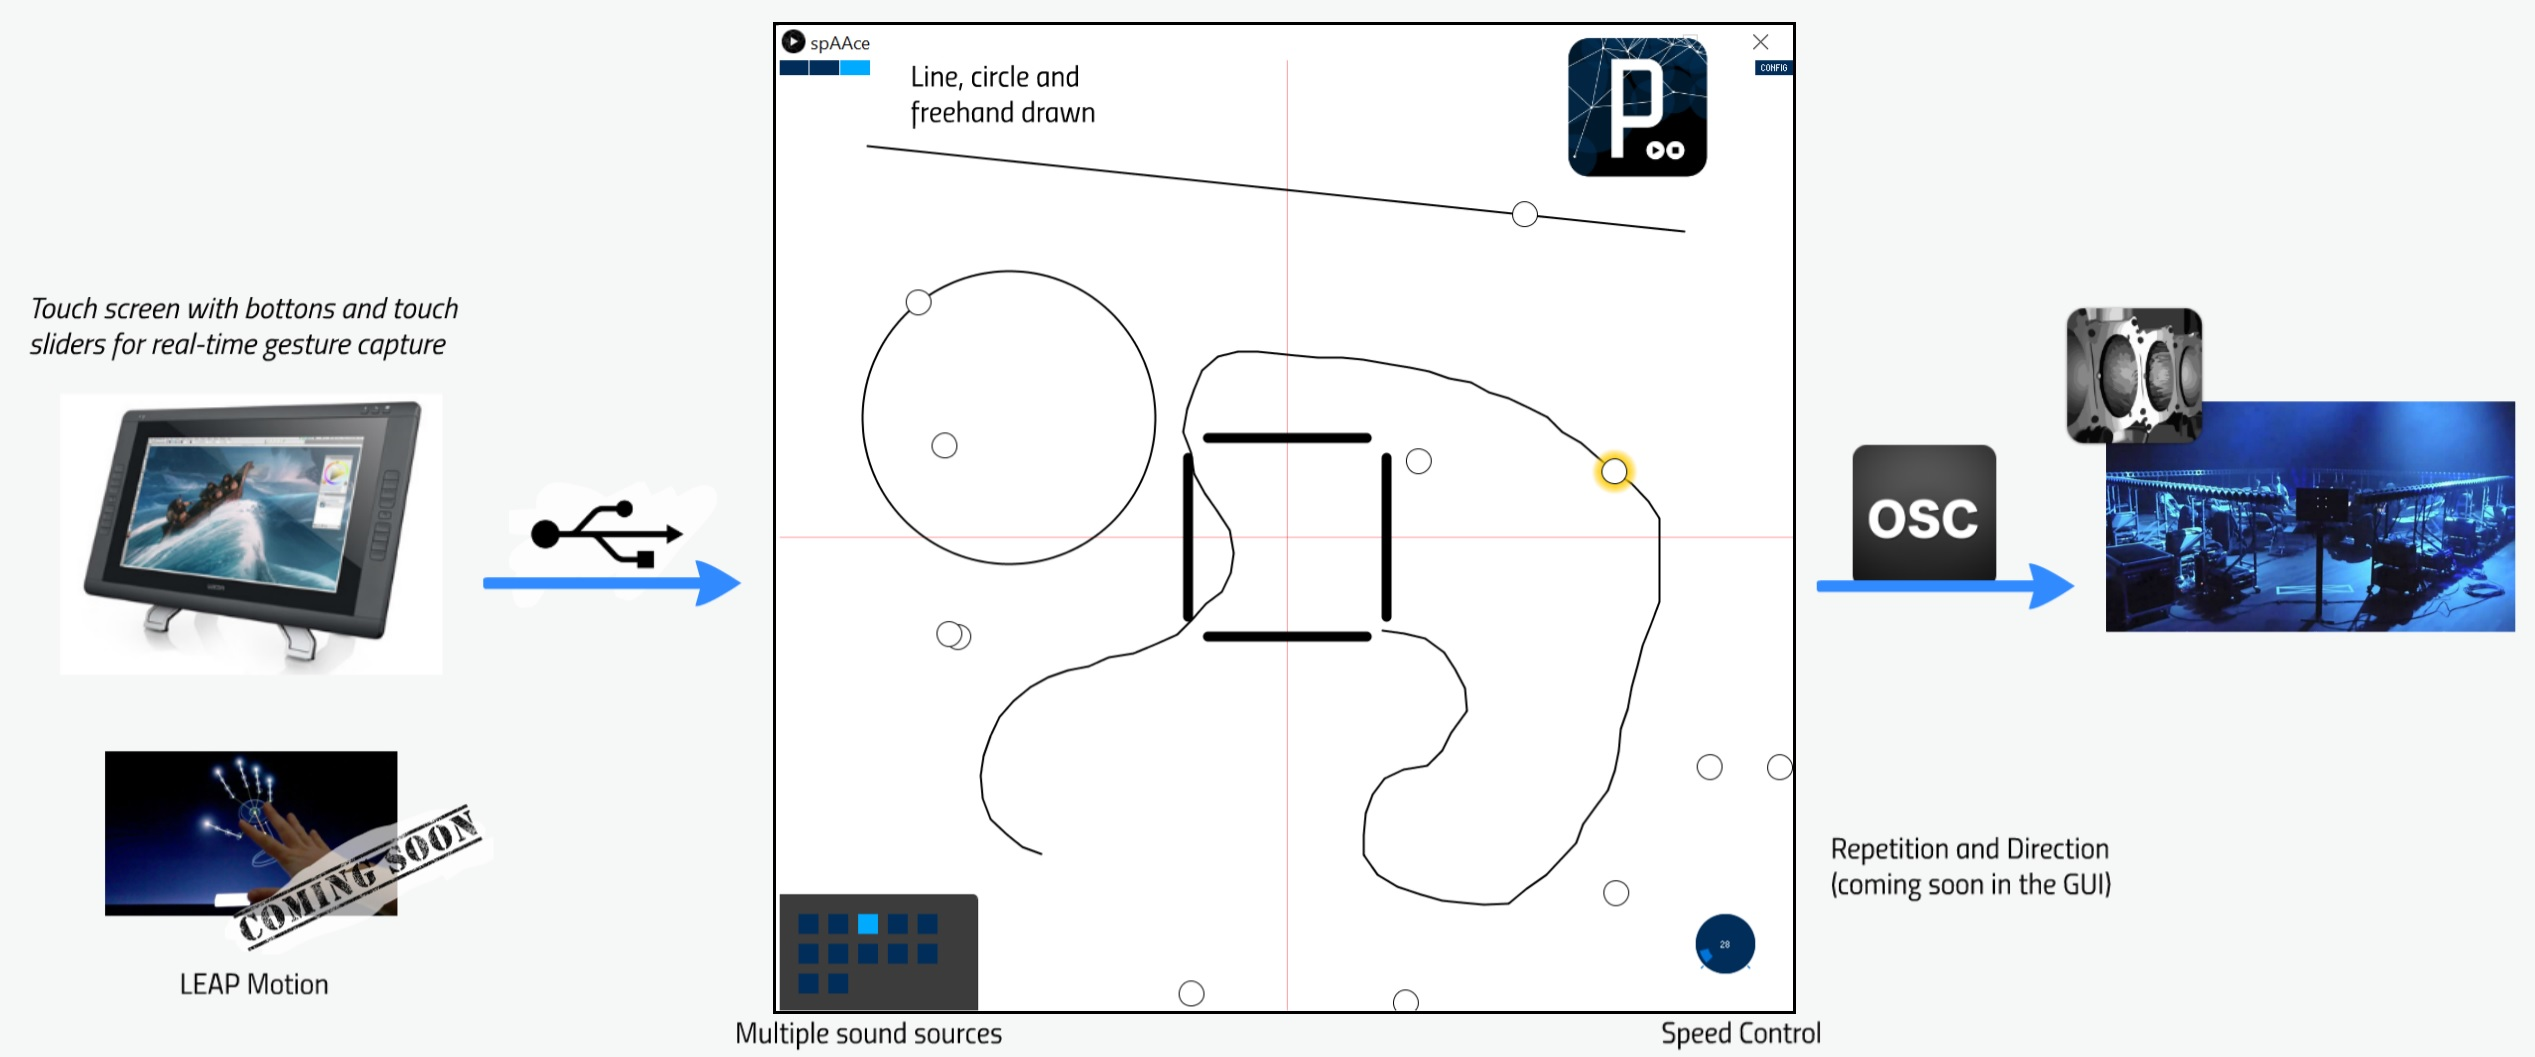
\includegraphics[scale = 0.2]{Architecture}
    \caption{The \textit{spAAce} architecture.}
    \label{fig:architecture}
\end{figure}


\section{Software architecture}
The graphical user interface has been developed to be controlled with a multi-touch screen like a tablet or similar. The interface allows the user to create and delete trajectories for the sound sources. There are three types of trajectories: 
\begin{itemize}
    \item line trajectory
    \item circular trajectory
    \item free hand drawing
\end{itemize}
These trajectories are displayed as buttons on the left upper side of the screen. The sound source can be dragged with a finger and when placed on top of one trajectory, it automatically follow the trajectory's path with a default speed. This speed can be changed with a knob on the bottom right side of the screen. Additionally, there is a control panel on the bottom left side of the screen where users can select each sound source. Lastly, since the OSC protocol is employed in order to communicate with WFSCollider the users can set the proper IP Address and OSC port by clicking on the `Network' button located on the right upper side of the screen.

%This speed among other properties can be changed in the sound source control panel on the bottom right part of the screen. For the user controls like the panel described before, controlP5 graphics library was used in Processing. Using this library we can display user controls for classical user interfaces, like buttons, knobs, radio buttons...etc.
\subsection{Device and Controller}
The controller is not fixed to a particular hardware since the development has been done in Processing, which is a multi-platform application. During testing sessions, a Wacom 22' multi-touch screen is being used. A Leap Motion will be used as controller in order to track hand movements and perform specific actions, for instance, moving sound sources towards a particular direction, applying spatial effects or even control more than one sound source at the same time. The controller is designed so that expression in terms of spatialization is improved as much as possible.

\section{Physical Setup}
Since \textit{spAAce} is a brand new project, it is continuously tested in the Multi-Sensory Experience laboratory of Aalborg University in Copenhagen. All the experiments have been conducted with the following set up: A WFS system of a square of 16 loudspeakers for each side; a computer running WFSCollider server for sound rendering (the OSC server); a laptop running the Processing sketch \emph{spAAce}, placed near the center of the WFS system and connected to the server via Ethernet (the OSC client); a Wacom Cintiq 22" touch standing in the center of the system as a input/output device for the client.


\section{Conclusion}
We presented a graphical application called \emph{spAAce} which let users control real-time movements of sound source by drawing trajectories. The first prototype of this application has been developed for a Wavefield Synthesis Systems and it is bound with WFSCollider, an open-source software based on Supercollider which lets users control such synthesis technique. In order to communicate with the software, Open Sound Control protocol has been employed. The \emph{spAAce} application has been implemented using Processing, a programming language for sketches and prototypes within the context of visual arts. This application aims to create a new way of interaction for live performance of spatial composition and live electronics.
Future work will focus on extending the application with a LEAP motion as 'expressive' input device in order to give a complete and interactive tool to composers and sound engineers. Understanding how this system can suite artists in real live performances will be a future improvement too.

\ifCLASSOPTIONcaptionsoff
  \newpage
\fi


\bibliographystyle{unsrt}
\bibliography{biblio}

\end{document}


